\documentclass[varwidth, border=10pt]{standalone}
\usepackage{tikz}
\usepackage[]{xcolor}
\usepackage{subcaption}
% % \usetikzlibrary{positioning}
% \usetikzlibrary{arrows,backgrounds}
% 
% \usepackage{amsmath, amsthm, amssymb}
% \input{commondefinitions}
% 	
% 
% 
% \begin{document}
% \pagestyle{empty}
% %\providecommand{\openone}{\leavevmode\hbox{\small1\kern-3.8pt\normalsize1}}
% 
% % \documentclass[12pt]{article}
% % \usepackage{psfrag}
% \usepackage{tikz}
% % \usetikzlibrary{positioning}
% % \usetikzlibrary{arrows,backgrounds}
 \usetikzlibrary{calc}
\usepackage{bbold}

\usepackage{tikz}
\usetikzlibrary{arrows}
\usetikzlibrary{quantikz}


\usepackage{amsmath, amsthm, amssymb}
\colorlet{coscolor}{blue}

\newcommand{\red}{\color{red}}
\newcommand{\blue}{\color{blue}}
%Colors

\definecolor{max}{rgb}{1,0.54,0.1}
\definecolor{medium}{rgb}{1,0.8,0.6}
\definecolor{min}{rgb}{1,0.9,0.8}
\begin{document}
\thispagestyle{empty}

\begin{figure} % {{{
\centering
\begin{subfigure}{0.9\textwidth}
\begin{subfigure}{.666\textwidth}
\centering
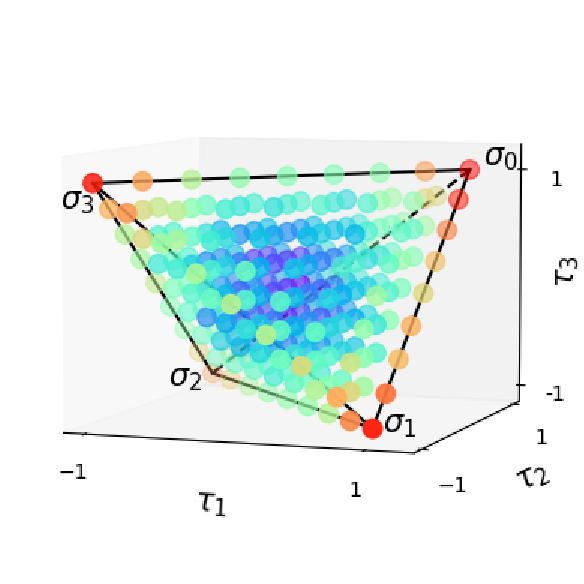
\includegraphics[width=.95\columnwidth]{tetra-def.pdf}
\end{subfigure}%
\begin{subfigure}{.333\textwidth}
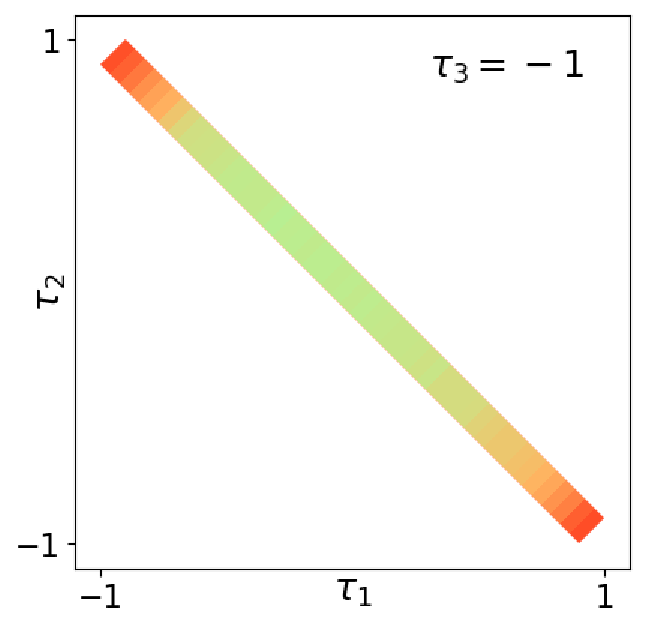
\includegraphics[width=.95\columnwidth]{corte1-2.pdf} \\
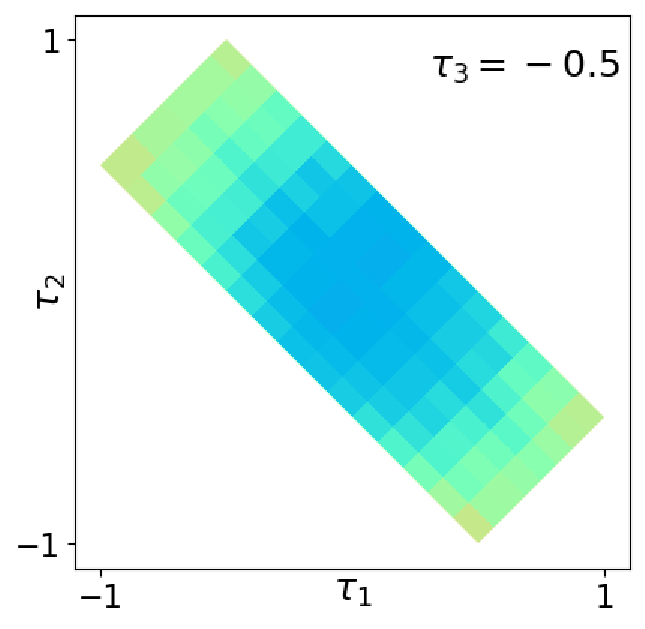
\includegraphics[width=.95\columnwidth]{corte2-2.pdf} \\
\end{subfigure}
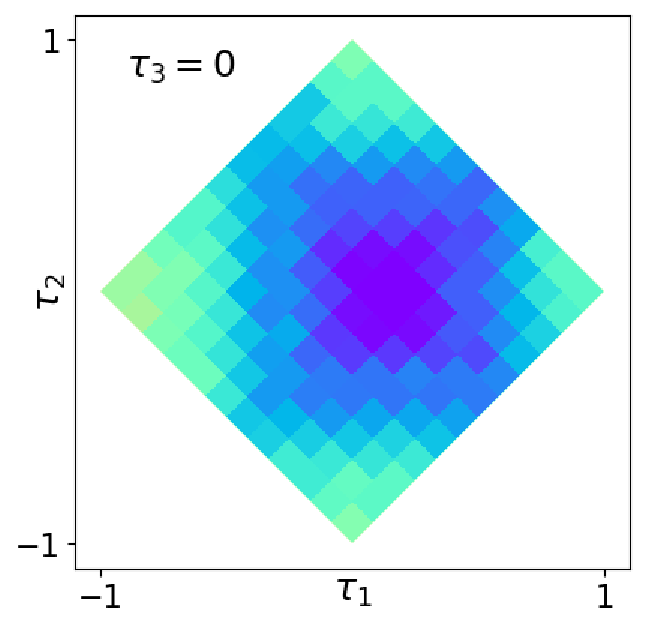
\includegraphics[width=.322\columnwidth]{corte3-2.pdf}
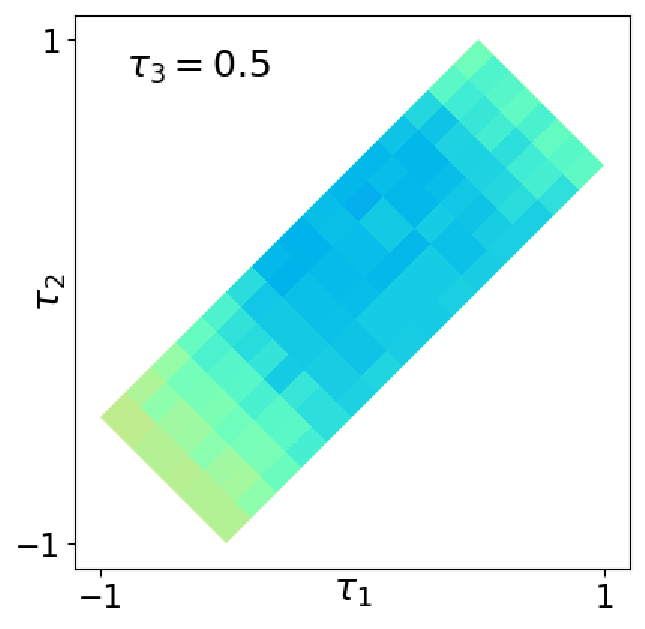
\includegraphics[width=.322\columnwidth]{corte4-2.pdf}
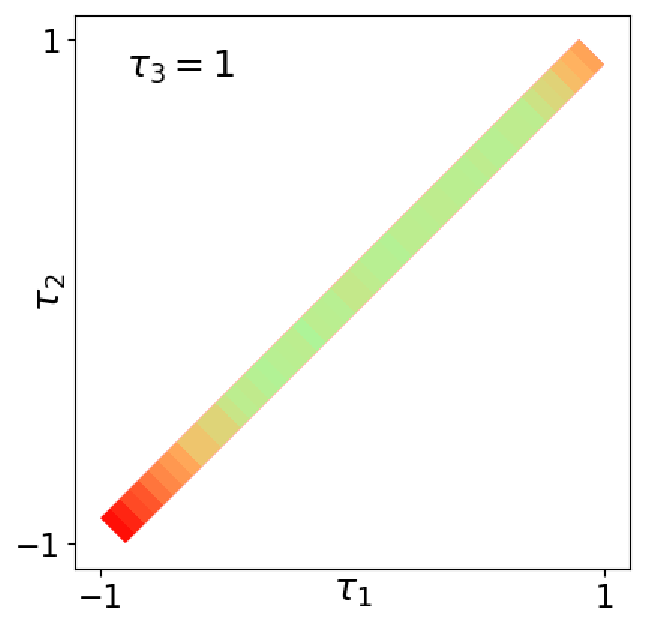
\includegraphics[width=.322\columnwidth]{corte5-2.pdf}
\end{subfigure}%
\begin{subfigure}{0.1\textwidth}
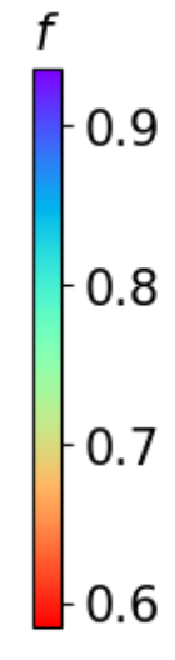
\includegraphics[width=.8\columnwidth]{col-2.pdf} \\ [2ex]
\end{subfigure}
%\caption{Results of the diamond fidelities as defined in \eref{eq:diamond-fid}
%for a sample of Pauli channels in the tetrahedron.  Notice that channels close
%to the center of the tetrahedron have high fidelities, while those close to the
%borders do not.  Moreover, we show the results for cuts of the tetrahedron at
%different values of $\tau_3$.}
%\label{Fig3}
\end{figure}

\end{document}



